\chapter{Fazit}
\section{Die Entwicklung einer KI-Ethik}
Die Entwicklung einer KI-Ethik ist ein wichtiger Schritt zur Förderung der verantwortungsvollen Entwicklung und Nutzung künstlicher Intelligenz. Organisationen wie die UNESCO und das Europäische Parlament haben KI-Ethikrichtlinien und -empfehlungen entwickelt, die auf Prinzipien wie Transparenz, Fairness, Datenschutz und sozialer Verantwortung basieren. Unternehmen wie IBM engagieren sich für die Entwicklung und Umsetzung ethischer KI-Praktiken, um sicherzustellen, dass KI zum Wohle der Gesellschaft eingesetzt wird.
\section{Fazit}
Künstliche Intelligenz kann unser tägliches Leben grundlegend verändern und verbessern, bringt aber auch ethische Herausforderungen und Risiken mit sich. Durch die verantwortungsvolle Entwicklung und Nutzung von KI können wir sicherstellen, dass diese Technologie ihr volles Potenzial entfaltet, um positive Veränderungen in unserer Gesellschaft zu bewirken.

\begin{figure}[h]
    \centering
    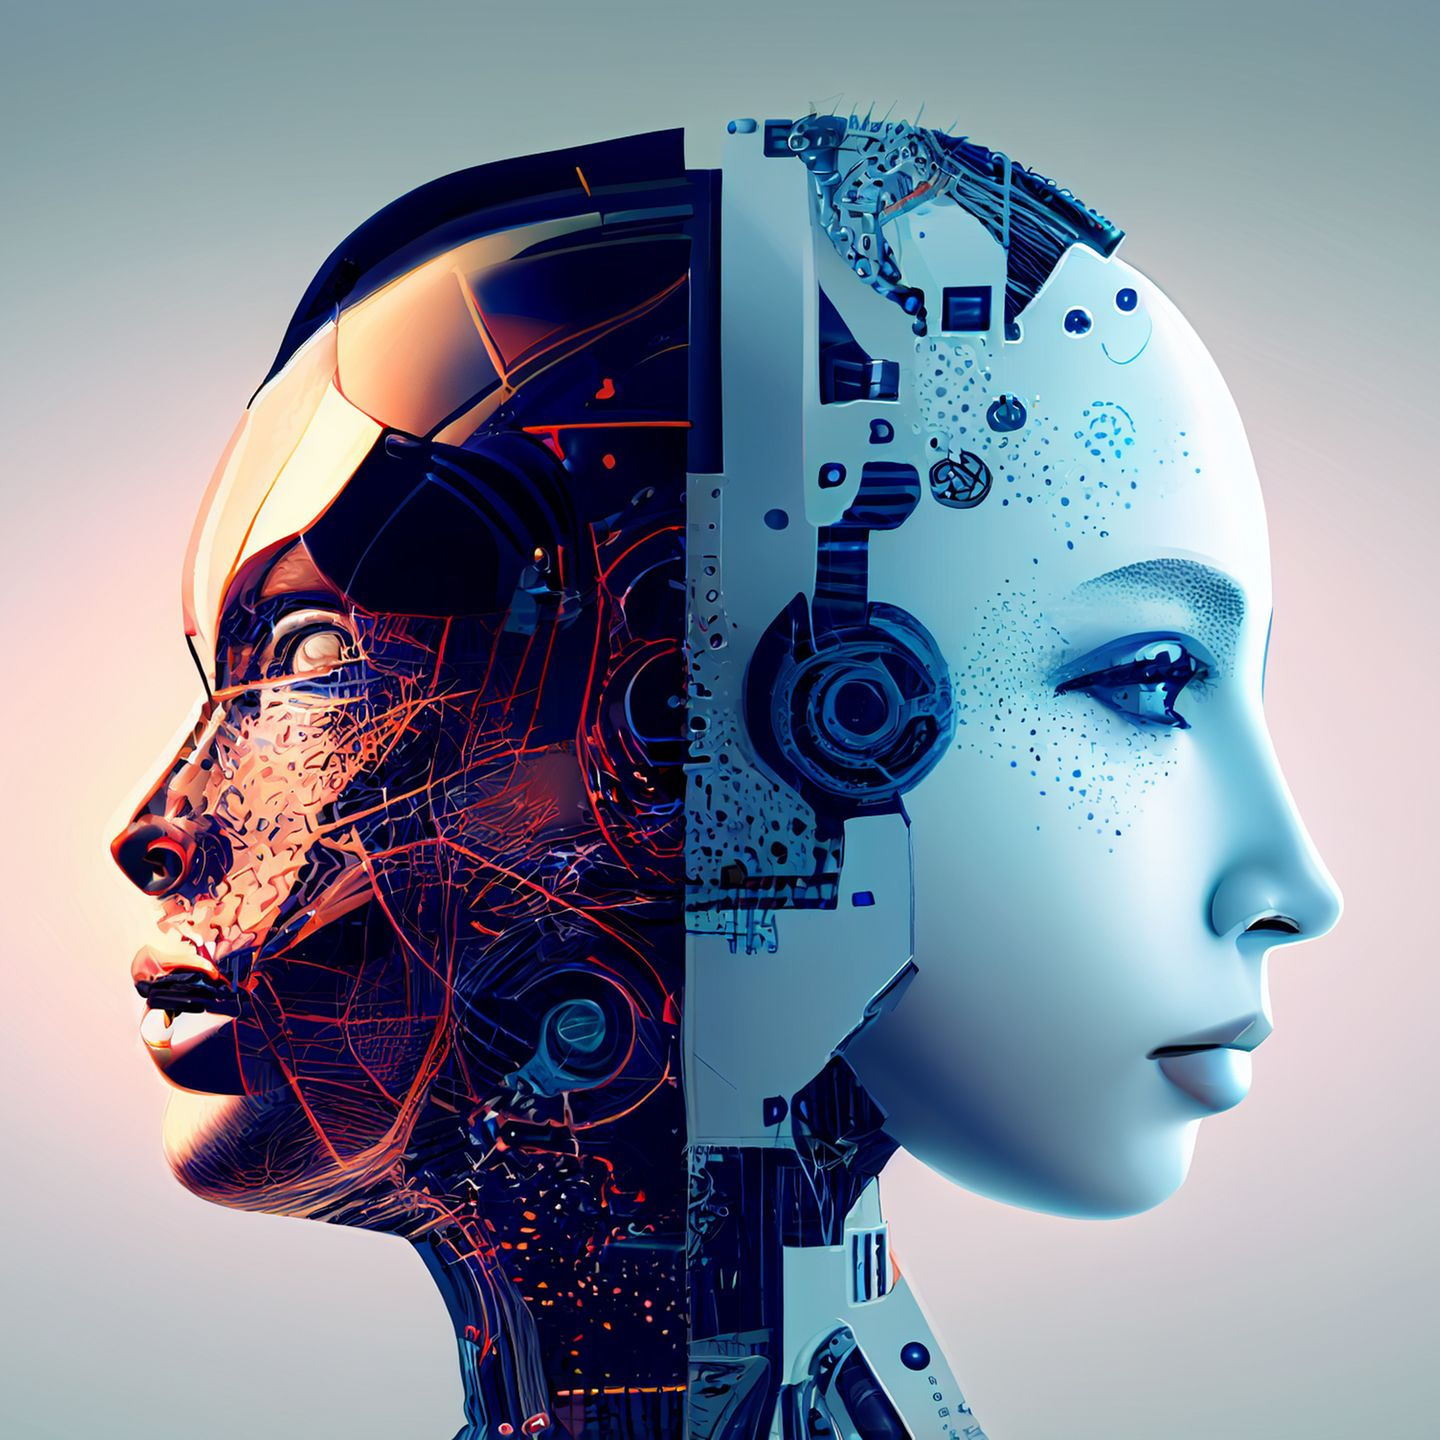
\includegraphics[width=0.4\textwidth]{KI bad good.jpg}
    \caption{ISt KI gefährlich?}
    \label{fig:ai2}
\end{figure}